In order to keep a good structure on the program and a logical separation of functionalities, several different data structures have been created. The main thought when designing the data structures was to enable easy access to all needed data for each stage in the pipeline each with different requirements and needs. The interfaces from Estimate3D provide such access to different arrangement of the same data, such as the 3D points, which have to be possible to both access and modify in several different steps of the pipeline.

\begin{figure}[htb]
	\centering
	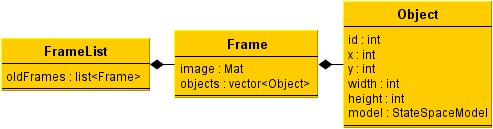
\includegraphics[width=110mm]{images/data_structures_uml.png}
	\caption{\textit{UML diagram of the main data structures. All estimated 3D-points of the model are shared between the necessary data structures, allowing for efficient updating of the 3D-points as well as efficient extraction of the most interesting data constellations used by Gold Standard, BA and Visualisation. Estimate3D act as the common interface to all data concerning the 3D model. It is of sorts a 'visibility function' for each camera, for each camera pair as well as for which cameras and their image coordinates observing a given 3D-point.}}
	\label{fig:UML_fig} %Skapar referens till figuren
\end{figure}

\subsubsection{PointPair, ObserverPair}
The point pair structure simply consists of two point pairs (cv::Point2d) from two different images that correspond to the same 3D point and the ObserverPair class contains one PointPair as well as pointers to the specific Cameras (see below) from which the PointPair originates. 

\subsubsection{Visible3DPoint}
This structure represents a point in 3D space. Apart from the coordinates for the point a list of all PointPairs observing it is stored as well.  \ref{fig:UML_fig}. %Figurreferens

\subsubsection{Camera}
The camera class represent a view of the 3D scene (an image). It contains information about what 3D points are visible in the image, and which image points these correspond to. Apart from this all necessary information about the camera itself is also stored here, such as internal parameters (K-matrix), rotation matrix and translation vector of the camera relative to the first camera is also stored in this class.

\subsubsection{CameraPair}
The camera pair is a data structure containing the Fundamental and Essential (F and E) matrices relating two cameras to each other. Beside this information the structure also contains pointers to each respective camera as well as vectors containing related PointPairs and pointers to corresponding 3D points.